\stepcounter{chapter} % This line will increment the chapter counter
\chapter*{Pattern Mining and Regression} % This line will create an unnumbered chapter
\addcontentsline{toc}{chapter}{\protect\numberline{\thechapter}Pattern Mining and Regression} % This line will add the chapter to your table of contents
\markboth{Pattern Mining and Regression}{} % This line will set the header
\vspace{-10mm}
\section{Regression}
\subsubsection*{Simple Regression}

\begin{comment}
\begin{wrapfigure}{r}{0.5\textwidth}
\centering
  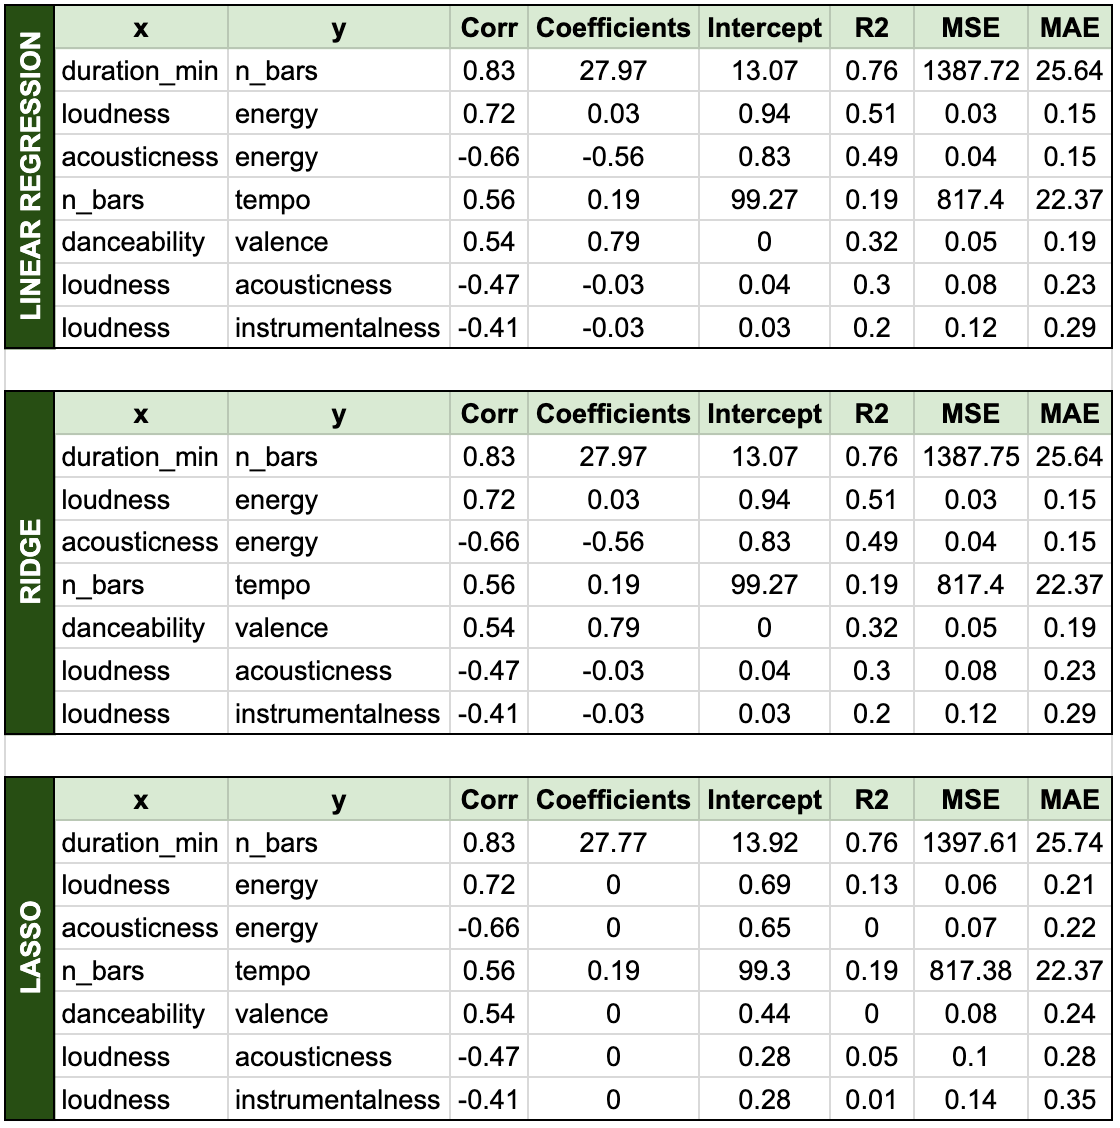
\includegraphics[width=.8\linewidth]{img/reg_1.png}
  \label{fig:test1}
  \centering
  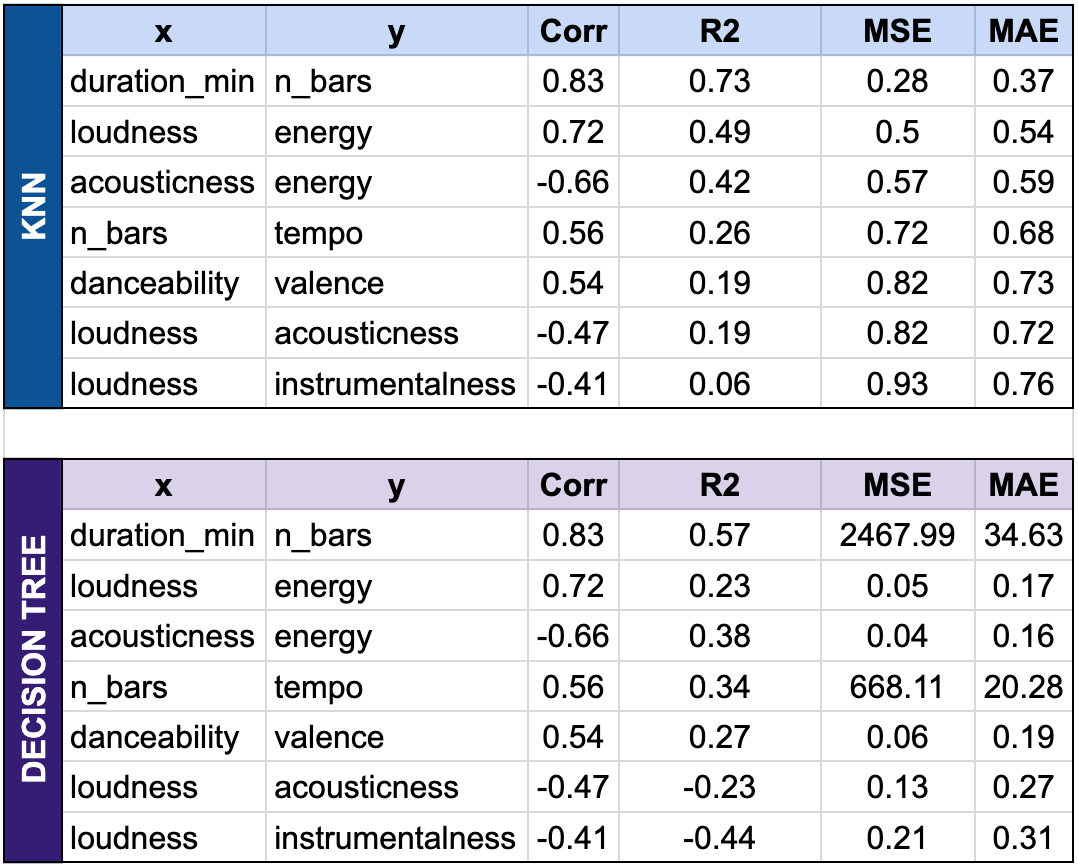
\includegraphics[width=.8\linewidth]{img/reg_2.png}
  \label{fig:test2}
\vspace{-1cm}
\end{wrapfigure}
\end{comment}

We created a function that performs simple linear regression using the provided regressor (that will be Linear, Ridge or Lasso) on the given training and testing datasets. It returns a dictionary containing the fitted model, its coefficients and intercept, and the $R^2$, $MSE$, and $MAE$ of the model on the test data. Then, for each regressor, our code performs a series of operations to identify pairs of features in a dataset that have a strong positive or negative correlation, and then applies simple linear regression to these pairs. After sorting the feature pairs based on the absolute value of their Spearman correlation coefficients, it filters the pairs to only include those with a correlation coefficient greater than $0.4$ or less than $-0.4$ (the threshold was chosen based on the values displayed in the correlation matrix). For each of these selected pairs, the code fits the model on the training data and uses it to predict the dependent variable in the test data. The list of results is converted into a pandas DataFrame that provides a comprehensive summary of the relationships between different features in the dataset and the performance of the model. In addition to the linear methods, we also used on the same pairs of features two previously seen models, KNN and DecisionTree, this time as regressors.
\begin{figure}[H]
\centering
\begin{minipage}{.5\textwidth}
  \centering
  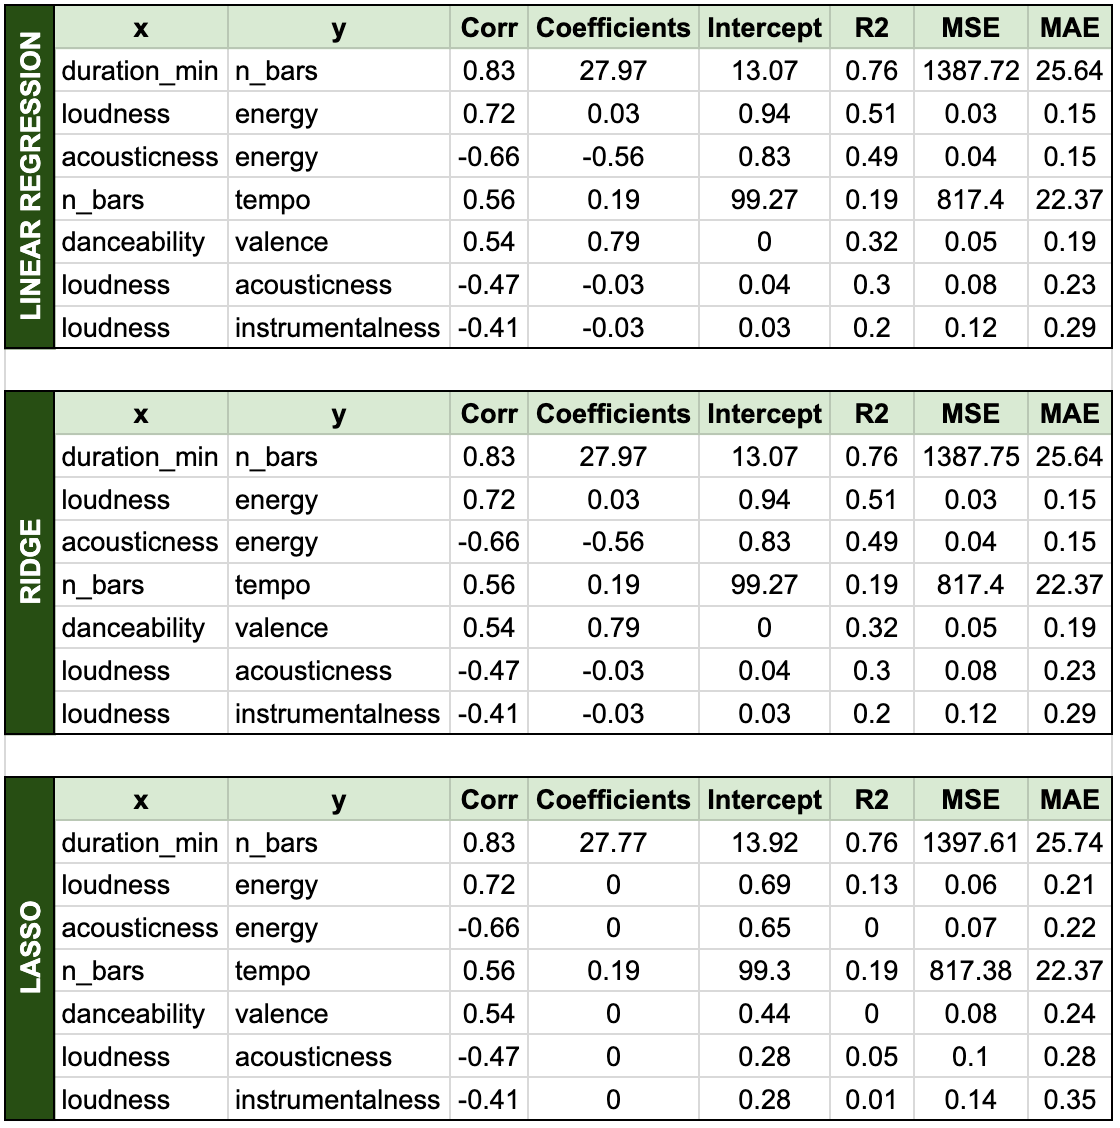
\includegraphics[width=.8\linewidth]{img/reg_1.png}
  \label{fig:test1}
\end{minipage}%
\begin{minipage}{.5\textwidth}
  \centering
  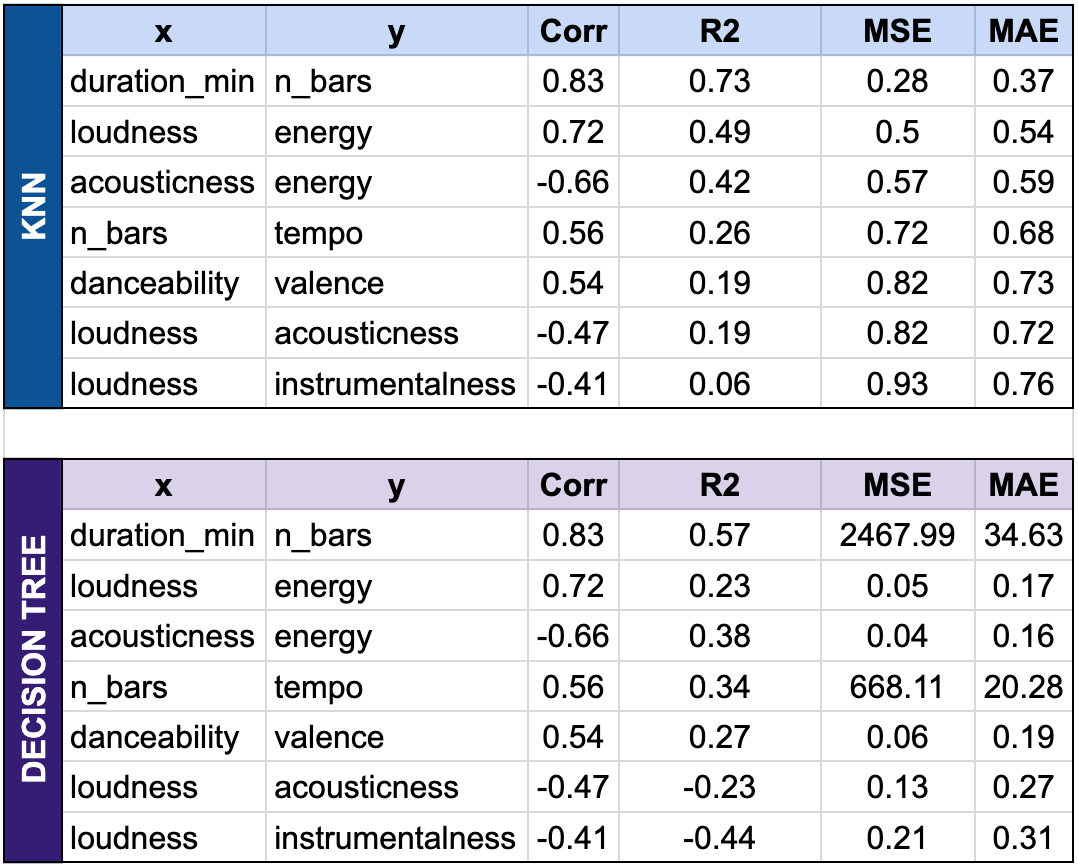
\includegraphics[width=.8\linewidth]{img/reg_2.png}
  \label{fig:test2}
\end{minipage}
\captionof{figure}{Results of linear and non-linear regression, performed on different pairs of features.}
\end{figure}
\noindent The best performing model is the one between duration\_min and n\_bars. This confirms what we expected, because the length of the song increases as the number of bars it contains increases. One of the worst performing models is the one between n\_bars and tempo. In fact, the number of bars in a song does not significantly influence its tempo, at least not in a linear way. The tempo and the number of beats of a song are largely independent musical elements: knowing the number of beats of a song does not provide much information about its tempo. The tempo of a piece is often chosen based on the mood or musical style, while the number of beats is typically determined by the structure and length of the piece.
\subsubsection{Multiple Regression}
We created a procedure that iterates over the list of targets containing only continuous variables of the dataset: the code, for each target, splits the dataset into train/test, standardizes the data, tests the different types of models seen above (performing a gridsearch based on the grid of parameters chosen) and then saves the results in a dataframe, sorting them by descending value of $R^2$.
\begin{figure}[H]
    \centering
    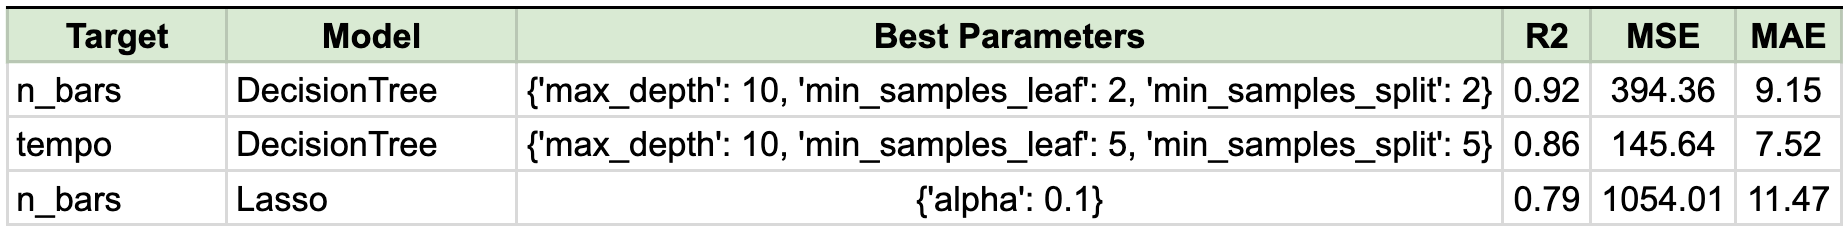
\includegraphics[scale=0.48]{img/multi_reg.png}
    \caption{Part of the results of multiple regression analysis: here we can see the 3 best combinations target-model.}
    \label{fig:enter-label}
\end{figure}
\subsubsection{Multivariate Regression}
As targets this time we have chosen: list \texttt{[popularity, danceability, energy]}, which can have implications in the music business, aiding in music recommendation, playlist creation, artist guidance, and advertising; then, after checking correlation to avoid multicollinearity, we added \texttt{[speechiness, acousticness, instrumentalness, liveness, valence]}, so that we can see performances with more targets.
\begin{figure}[H]
    \centering
    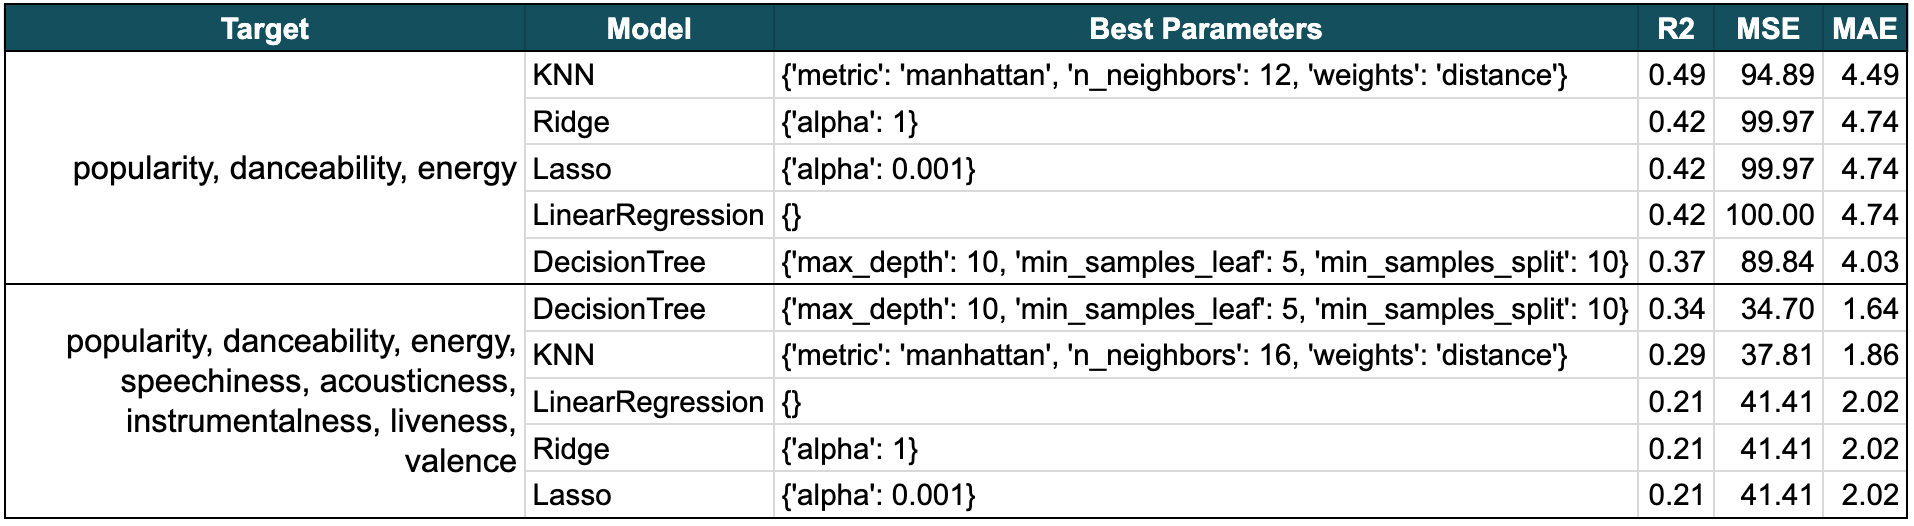
\includegraphics[scale=0.45]{img/multivariate.png}
    \caption{Results of the multivariate regression analysis.}
    \label{fig:enter-label}
\end{figure}
\section{Pattern Mining}
Before starting the analysis, we prepared the data: we mapped the categorical features to the actual values, for example, by substituting each key value for the corresponding Pitch Class Notation value (1 represents $C$ pitch, 2 represents $C\sharp/D\flat$, and so on); then we discretized the continuous variables, each in 3 bins, using \texttt{pd.cut}.
\subsection{Frequent Patterns}
\subsubsection*{Apriori}
Before running the Apriori algorithm, we looked for the optimal values of supp (minimum support of an item set) and zmin (minimum number of items per item set). The code defines a grid of parameters for the Apriori algorithm: \texttt{supp} values are generated using numpy’s linspace function to create 5 evenly spaced values between 10 and 50; \texttt{zmin} values are generated using numpy’s arange function to create a range of values from 5 to the number of columns in the dataframe. Then it runs the Apriori algorithm for each combination of \texttt{supp} and \texttt{zmin} values in the parameter grid, computing, for each combination, the number of frequent, closed, and maximal itemsets. Results are sorted by the number of frequent, closed, and maximal itemsets in descending order. The best configuration founded is \texttt{[supp=10, zmin=5]}. In fact, by setting 2, 3 or 4 as the minimum of the \texttt{zmin} range, we realized that the patterns found were just a simple confirmation of some information already found in data understanding: for example, in the dataset most of the tracks have a fairly short duration (the distribution is positively skewed). By setting a value of zmin equal to 5 instead, we can already begin to get more useful patterns.
\begin{figure}[H]
\centering
\begin{minipage}{.5\textwidth}
\centering
    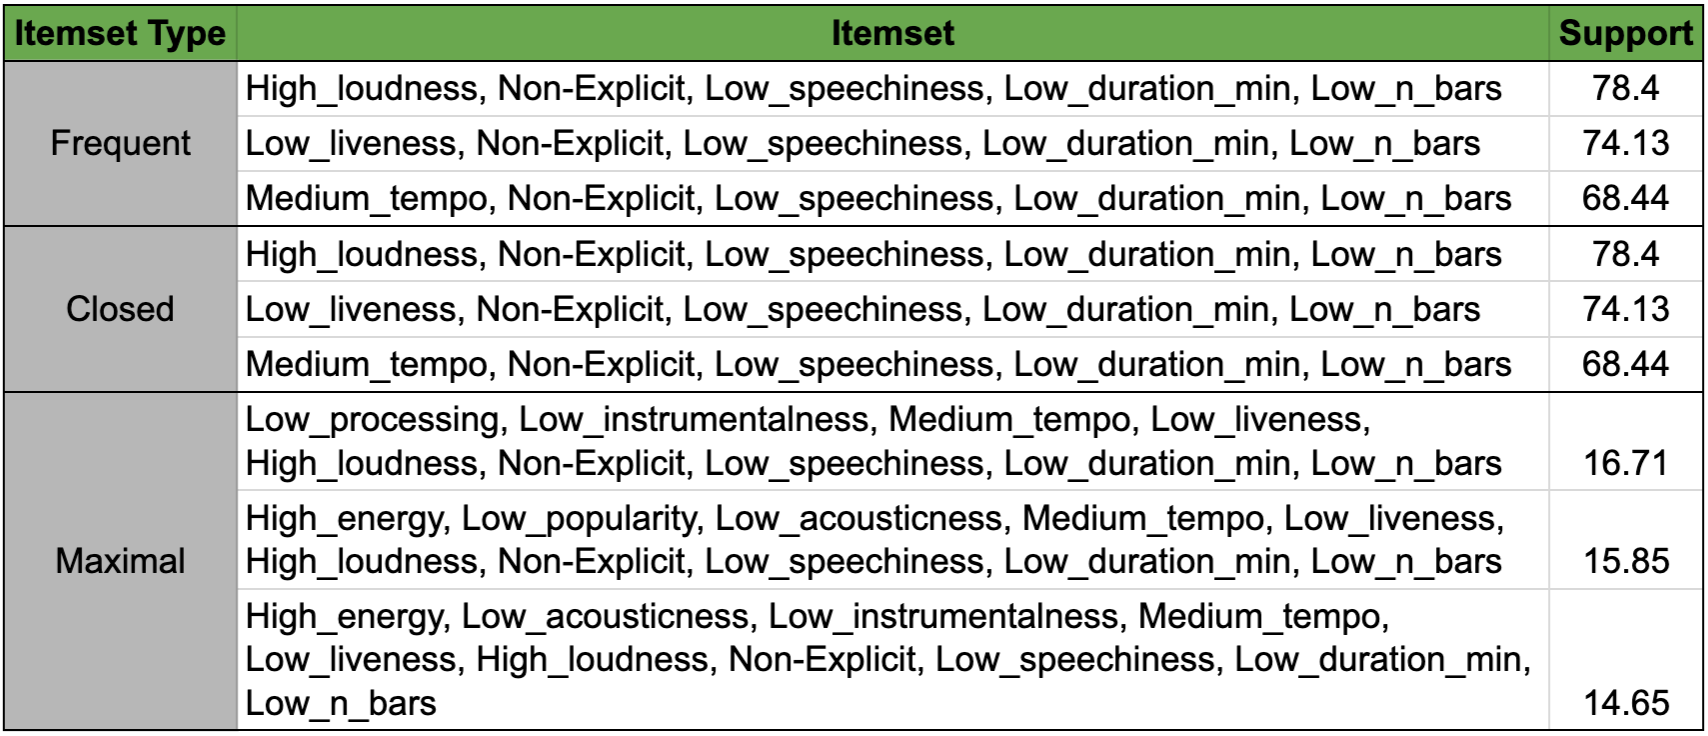
\includegraphics[width=\linewidth]{img/freqclosmax.png}
    \caption{Highest support values for the frequent, closed, and maximal itemsets derived from the Apriori algorithm.}
    \label{fig:enter-label}
\end{minipage}%
\hspace{0.5cm}
\begin{minipage}{.4\textwidth}
  \centering
  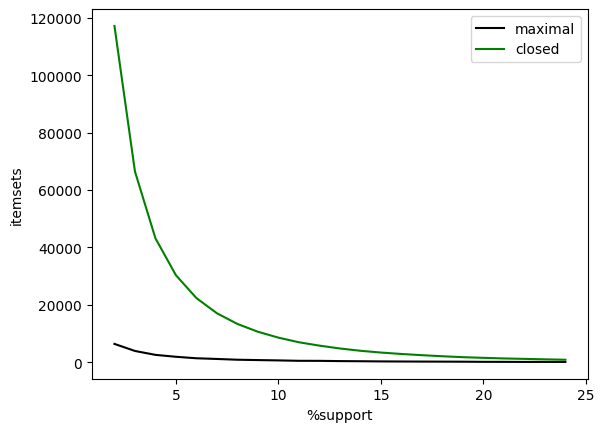
\includegraphics[width=.8\linewidth]{img/maxclos_plot.png}
  \caption{Number of maximal and closed itemsets (y-axis) for different support thresholds (x-axis).}
  \label{fig:test2}
\end{minipage}
\end{figure}
\noindent Our dataset predominantly consists of non-explicit tracks with high volume, low speechiness, a duration range that remains below 22 minutes, and a low number of bars. Tracks with medium tempo and low speechiness also have a significant presence. The presence of liveness feature among the most frequent patterns also suggests that dataset contains lots of tracks that have a low “live” feel.
\subsubsection*{FP-Growth}
We implemented the same procedure used for apriori, with the goal of finding the optimal values of supp and zmin, which are again \texttt{[supp=10, zmin=5]}. These are the three frequent patterns found with the highest support:\\
\begin{center}
\tiny{
\begin{tabular}[ht]
{|l|c|}
\hline
\textbf{Frequent Itemset} & \textbf{Support} \\
\hline
High\_loudness, Non-Explicit, Low\_speechiness, Low\_duration\_min, Low\_n\_bars & 78.4 \\
Low\_liveness, Non-Explicit, Low\_speechiness, Low\_duration\_min, Low\_n\_bars & 74.13 \\
Low\_liveness, High\_loudness, Low\_speechiness, Low\_duration\_min, Low\_n\_bars & 67.97 \\
\hline
\end{tabular}
}
\end{center}
\subsection{Association Rules}
We implemented a code that runs the Apriori algorithm for association rule mining over a range of confidence values (from 50 to 95) with a step of 5. For each \texttt{conf} value we then compute the average lift for the rules generated. We chose as optimal \texttt{conf} value the confidence level with the highest average lift. Finally, the code runs the Apriori algorithm again with the best confidence level and displays the resulting association rules sorted by lift in descending order.
\begin{figure}[H]
    \centering
    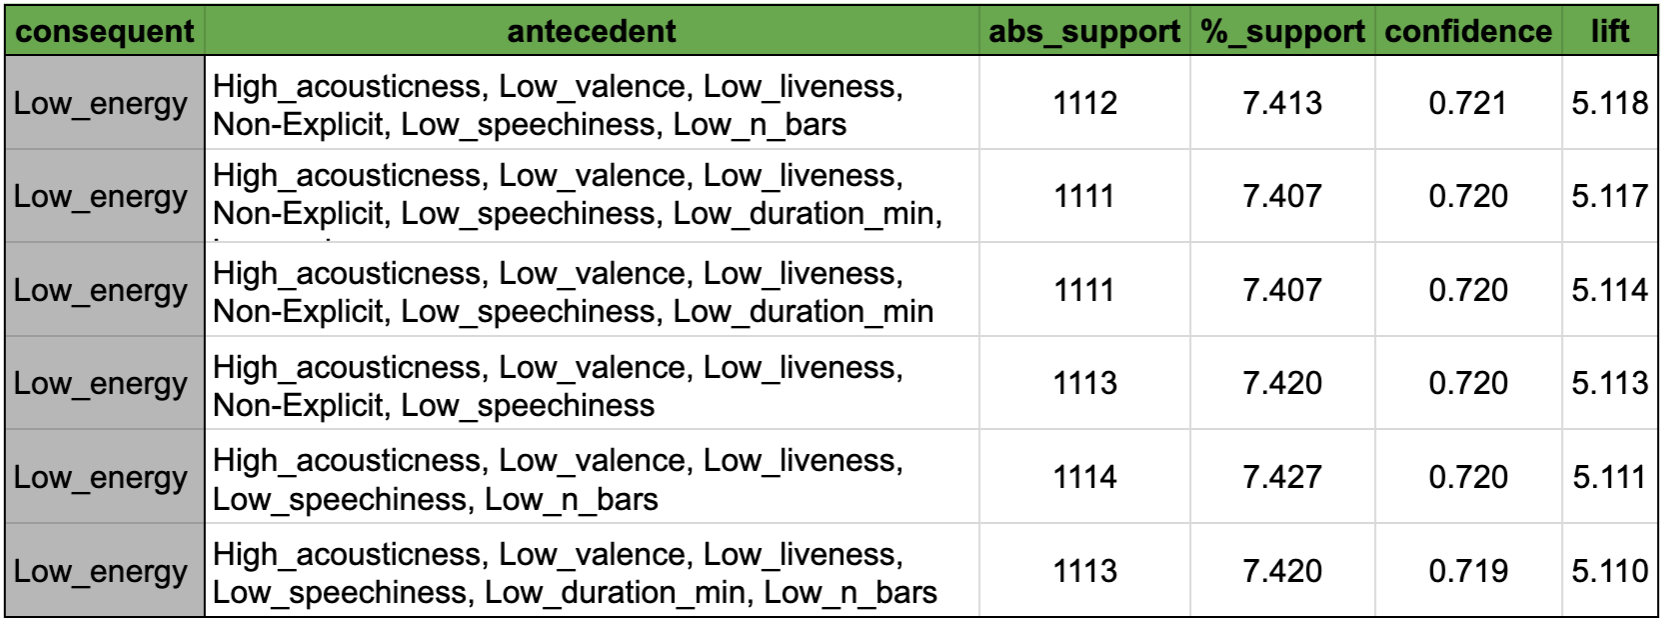
\includegraphics[scale=0.5]{img/rules.png}
    \caption{Association rules sorted by lift.}
    \label{fig:enter-label}
\end{figure}
We can see the following information:
\begin{itemize}
    \item Consequents: in our case it's mainly related to `energy`.
    \item Confidence: measures how often the rule has been found to be true. For example, a confidence of 0.72 for the first rule means that in about 72\% of the transactions containing [High\_acousticness, Low\_valence, Low\_liveness, Non-Explicit, Low\_speechiness, Low\_n\_bars] appear to have a low energy level.
    \item lift: ratio of the observed support to that expected if the antecedent and the consequent were independent. In our case, all the higher lifts are around 5, which means that the rules are quite significant.
\end{itemize}

The first rule can be read as: “If a relatively short song is acoustic, non-expicit and has low valence, liveness, speechiness, then it’s likely to have a low energy". This rule has a confidence of about 72\% and is about 5.1 times as likely to occur as would be expected if the conditions and result were independent. This pattern repeats for the other rules with slight variations in the conditions. All this also confirms the study of data understanding, in which we assumed such relationships based more or less only on correlations.